% Copyright 2004 by Till Tantau <tantau@users.sourceforge.net>.
%
% In principle, this file can be redistributed and/or modified under
% the terms of the GNU Public License, version 2.
%
% However, this file is supposed to be a template to be modified
% for your own needs. For this reason, if you use this file as a
% template and not specifically distribute it as part of a another
% package/program, I grant the extra permission to freely copy and
% modify this file as you see fit and even to delete this copyright
% notice.

\documentclass{beamer}

% There are many different themes available for Beamer. A comprehensive
% list with examples is given here:
% http://deic.uab.es/~iblanes/beamer_gallery/index_by_theme.html
% You can uncomment the themes below if you would like to use a different
% one:
%\usetheme{AnnArbor}
%\usetheme{Antibes}
%\usetheme{Bergen}
%\usetheme{Berkeley}
%\usetheme{Berlin}
%\usetheme{Boadilla}
%\usetheme{boxes}
%\usetheme{CambridgeUS}
%\usetheme{Copenhagen}
%\usetheme{Darmstadt}
%\usetheme{default}
%\usetheme{Frankfurt}
%\usetheme{Goettingen}
%\usetheme{Hannover}
%\usetheme{Ilmenau}
%\usetheme{JuanLesPins}
%\usetheme{Luebeck}
\usetheme{Madrid}
%\usetheme{Malmoe}
%\usetheme{Marburg}
%\usetheme{Montpellier}
%\usetheme{PaloAlto}
%\usetheme{Pittsburgh}
%\usetheme{Rochester}
%\usetheme{Singapore}
%\usetheme{Szeged}
%\usetheme{Warsaw}

\usepackage[brazilian]{babel}
\usepackage[utf8]{inputenc}
\usepackage[T1]{fontenc}

\title{Reconstrução de objetos 3D a partir de imagens}

% A subtitle is optional and this may be deleted
\subtitle{aplicado a medicina}

\author{Marlon H. Schweigert\inst{1} \and Roberto S. Rosso\inst{1}}
% - Give the names in the same order as the appear in the paper.
% - Use the \inst{?} command only if the authors have different
%   affiliation.

\institute[UDESC] % (optional, but mostly needed)
{
  \inst{1}%
  UDESC\\
  Universidade do Estado de Santa Catarina
}
% - Use the \inst command only if there are several affiliations.
% - Keep it simple, no one is interested in your street address.

\date{Automação e Controle, 2018.1}
% - Either use conference name or its abbreviation.
% - Not really informative to the audience, more for people (including
%   yourself) who are reading the slides online

\subject{Reconstrução 3D para medicina}
% This is only inserted into the PDF information catalog. Can be left
% out. 

% If you have a file called "university-logo-filename.xxx", where xxx
% is a graphic format that can be processed by latex or pdflatex,
% resp., then you can add a logo as follows:

% \pgfdeclareimage[height=0.5cm]{university-logo}{university-logo-filename}
% \logo{\pgfuseimage{university-logo}}

% Delete this, if you do not want the table of contents to pop up at
% the beginning of each subsection:
\AtBeginSubsection[]
{
  \begin{frame}<beamer>{Outline}
    \tableofcontents[currentsection,currentsubsection]
  \end{frame}
}

% Let's get started
\begin{document}

\begin{frame}
  \titlepage
\end{frame}

\begin{frame}{Roteiro}
  \tableofcontents
  % You might wish to add the option [pausesections]
\end{frame}

% Section and subsections will appear in the presentation overview
% and table of contents.
\section{Introdução}

\subsection{Objetivo}
\subsection{Temas}

\begin{frame}{Temas}{}
  \begin{itemize}
  \item {
    Aceleração de algoritmos de reconstrução usando GPU.
  }
  \item {
    Detecção de câncer de mama.
  }
  \item {
    Auxilio visual para procedimentos cirúrgicos.
  }
  \item {
    Reconstrução de ossos da região pélvica a partir de imagens de tomografia.
  }
  \end{itemize}
\end{frame}

\section{Artigos}

\subsection{GPU para reconstrução 3D}

\begin{frame}{Agilizar o processo de criação de nuvens de pontos}
  \begin{itemize}
  \item {
    Processamento de dados massivos.
  }
  \item {
    Serviço de geração de malhas a partir de imagens.
  }
  \end{itemize}
\end{frame}


\subsection{Reconhecimento de câncer de mama}

\begin{frame}{Método de processamento}
  \begin{itemize}
  \item {
    Obter dados com tomografia.
  }
  \item {
   Tratar imagens a fim de destacar o sistema nervoso danificado.
  }
  \item {
    Gerar nuvem de pontos.
  }
  \item {
   Gerar malha.
  }
  \end{itemize}
\end{frame}

\begin{frame}{Tomografia}
    \begin{figure}[htb]
    \label{fig:contraste}
    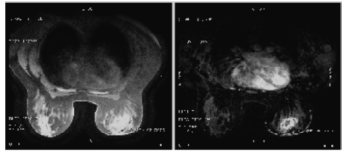
\includegraphics[width=6cm]{./img/contraste.png}
    \centering
    \end{figure}
\end{frame}

\begin{frame}{Nuvem de pontos}
    \begin{figure}[htb]
    \label{fig:reconstrucao}
    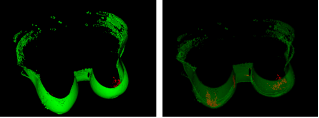
\includegraphics[width=6cm]{./img/reconstrucao.png}
    \centering
    \end{figure}
\end{frame}

\begin{frame}{Reconstrução}
    \begin{figure}[htb]
    \label{fig:final}
    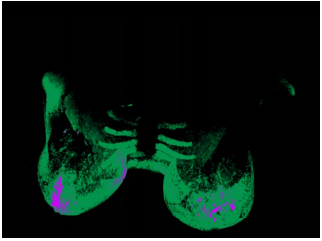
\includegraphics[width=6cm]{./img/final.png}
    \centering
    \end{figure}
\end{frame}

\subsection{Reconstrução de ossos da região pélvica}

\begin{frame}{Método de processamento}
  \begin{itemize}
  \item {
    Obter dados com tomografia.
  }
  \item {
   Tratar imagens a fim de remover ruído.
  }
  \item {
    Gerar nuvem de pontos.
  }
  \item {
   Gerar malha.
  }
  \end{itemize}
\end{frame}

\begin{frame}{Obter dados}
 \begin{figure}[htb]
\label{fig:pelvis_contraste}
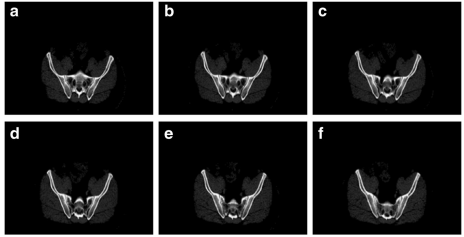
\includegraphics[width=6cm]{./img/pelvis_contraste.png}
\centering
\end{figure}
\end{frame}

\begin{frame}{Tratamento de imagem}
\begin{figure}[htb]
\label{fig:pelvis_reconstrucao}
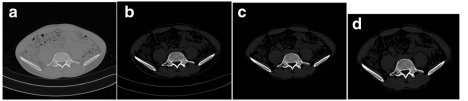
\includegraphics[width=6cm]{./img/pelvis_reconstrucao.png}
\centering
\end{figure}
\end{frame}


\begin{frame}{Resultado final}
\begin{figure}[htb]
\label{fig:pelvis_final}

\includegraphics[width=6cm]{./img/pelvis_final.png}
\centering
\end{figure}
\end{frame}

\subsection{Ultrassom 3D para câncer de mama}

\begin{frame}{Método de processamento}
  \begin{itemize}
  \item {
    Obter imagens pelo ultrassom
  }
  \item {
   tratar imagens
  }
  \item {
    Gerar fatiamento das imagens geradas
  }
  \end{itemize}
\end{frame}

\begin{frame}{Implantação}
  \begin{figure}[htb]
    \label{fig:implantacao}
    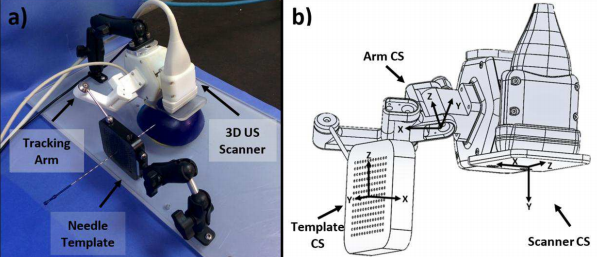
\includegraphics[width=6cm]{./img/implantacao.png}
    \centering
    \end{figure}
\end{frame}

\begin{frame}{Resultado final}
    \begin{figure}[htb]
    \label{fig:scanner3d_final}
    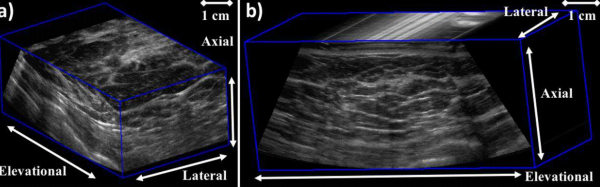
\includegraphics[width=6cm]{./img/scanner3d_final.png}
    \centering
    \end{figure}
\end{frame}


\subsection{Laparoscópico 3D}

\begin{frame}{Método de processamento}
  \begin{itemize}
  \item {
    Hardware para obter dados em tempo real (1.72 FPS).
  }
  \item {
    Obter imagem 2D e nuvem de pontos.
  }
  \item {
    Exibir imagem tratada, nuvem de pontos e imagem real.
  }
  \end{itemize}
\end{frame}

\begin{frame}{Implantação}
    \begin{figure}[htb]
\label{fig:laparoscopico}
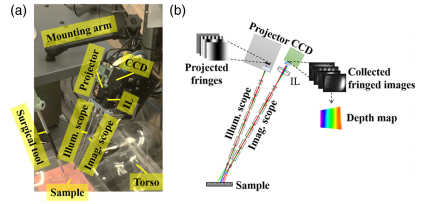
\includegraphics[width=6cm]{./img/laparoscopico.png}
\centering
\end{figure}
\end{frame}

\begin{frame}{Distância obtida}
\begin{figure}[htb]
\label{fig:distancia}
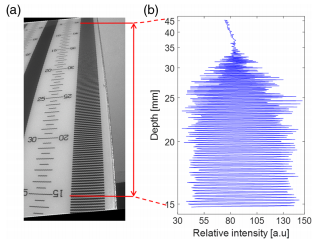
\includegraphics[width=6cm]{./img/distancia.png}
\centering
\end{figure}
\end{frame}

\begin{frame}{Resultado final}
\begin{figure}[htb]
\label{fig:laparo_final}
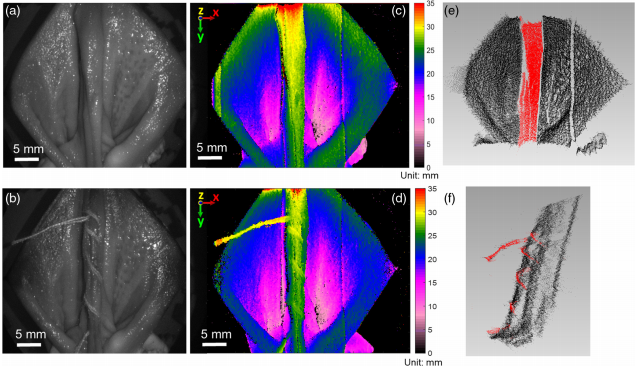
\includegraphics[width=6cm]{./img/laparo_final.png}
\centering
\end{figure}
\end{frame}
% All of the following is optional and typically not needed. 
\appendix
\section<presentation>*{\appendixname}
\subsection<presentation>*{For Further Reading}

\begin{frame}[allowframebreaks]
  \frametitle<presentation>{For Further Reading}
    
  \begin{thebibliography}{10}
    
  \beamertemplatebookbibitems
  % Start with overview books.


  \beamertemplatearticlebibitems
  \bibitem{A}
    Yu, Hui and Wang, Haijun and Shi, Yao and Xu, Ke and Yu, Xuyao and Cao, Yuzhen
    \newblock {The segmentation of bones in pelvic CT images based on extraction of key frames}.
    
\bibitem{A}
    Xu, Tao and Sun, Kun and Tao, Wenbing
    \newblock {GPU Accelerated Cascade Hashing Image Matching for Large Scale 3D Reconstruction}.
    
\bibitem{A}
    Abdul{\textendash}Kreem, Luma Issa
    \newblock {Depth Estimation and Shape Reconstruction of a 2D Image Using N.N. and Bezier Surface Interpolation}.

\bibitem{A}
    Gnonnou, Christo and Smaoui, Nadia
    \newblock {Segmentation and 3D reconstruction of MRI images for breast cancer detection}.

\bibitem{A}
Michael, Justin and Morton, Daniel and Batchelar, Deidre and Hilts, Michelle and Crook, Juanita and Fenster, Aaron
    \newblock {Development of a 3D Ultrasound Guidance System for Permanent Breast Seed Implantation}.

\bibitem{A}
Le, Hanh N. D. and Nguyen, Hieu and Wang, Zhaoyang and Opfermann, Justin and Leonard, Simon and Krieger, Axel and Kang, Jin U.
    \newblock {Demonstration of a laparoscopic structured-illumination three-dimensional imaging system for guiding reconstructive bowel anastomosis}.

  \end{thebibliography}
\end{frame}

\end{document}


